\documentclass[journal,12pt,twocolumn]{IEEEtran}
\parindent 0px
\usepackage{setspace}
\usepackage{graphicx}
\usepackage{enumitem}
\usepackage{amsmath}

\title{Assignment 1 \\ \Large AI1110: Probability and Random Variables \\ }
\author{Pericherla Pranav Varma \\ \normalsize CS21BTECH11044 \\ \vspace*{20pt} \normalsize  06 April 2022 \\ \vspace*{20pt} \Large ICSE 2017 Grade 10}
\begin{document}
\maketitle
\doublespacing
Question 3(c):\\
The marks of 10 students of a class in an examination arranged in ascending order
is as follows:\\
13, 35, 43, 46, x, x+4, 55, 61, 71, 80.\\
If the median marks is 48, find the value of x. Hence find the mode of the given
data.\\[9pt]
\textbf{Solution}:\\[8pt]
Required: 
\begin{enumerate}[label=(\roman*)]	
	\item value of $x$.
	\item mode of the data.
\end{enumerate}

Median(definition): it is the middle number in a sorted ordered list of number. \\
i.e., if $n$ be the number of entries in given data\\
then median of the data is:\\
\begin{enumerate}[label=(\roman*)]
\item if $n$ = odd, Median = $(\frac{n}{2})^{th}$ element.\\
\item if ($n$ = even), Median = average of $(\frac{n}{2})^{th}$ and $(\frac{n+1}{2})^{th}$ elements.\\[6pt]
\end{enumerate}
As, Here the value of n is \underline{odd}.\\
	therefore,\\
	\begin{align}
	Median &= \dfrac{(x)+(x+4)}{2}.\\
	  Median &= \dfrac{(2x+4)}{2}.\\
	 Median &= x+2.\\
	 x &= Median-2\\
	 x&=48-2\\
	 x&=46.
	\end{align}	
	therefore, $ \underline{x=46.}$ \\[10pt]
Requirement (ii) : mode of the data.(Histogram) \\[4pt]
Converting given set of sorted numbers into Class Intervals(to use Histogram method to find mode):\\[12pt]

Given data :13, 35, 43, 46, 46, 50, 55, 61, 71, 80.\\ [12pt]
CONVERTED Class intervals and frequency table:\\[16pt]

%table
\begin{table}[h]
    \centering
		\begin{tabular}{|c|c|}
	\hline
	\textbf{Class Interval} & \textbf{frequency} \\ 
	\hline
	0-10 & 0 \\
	\hline
	10-20 & 1 \\
	\hline
	20-30 & 0 \\
	\hline
	30-40 & 1 \\
	\hline
	40-50 & 3 \\
	\hline
	50-60 & 2 \\
	\hline
	60-70 & 1 \\
	\hline
	70-80 & 2 \\
	\hline
	\end{tabular} 
    \caption{}
    \label{TABLE}
\end{table}
%graph
\begin{figure}
	\centering
	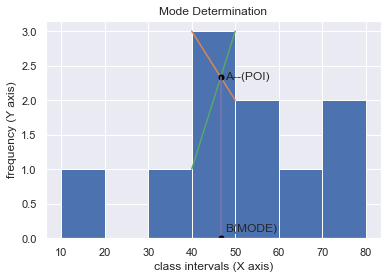
\includegraphics[scale=0.8]{graph.png}
	\caption{Graph}
\end{figure}	
Hence, Mode(approx) of given data = 46.66\\
i.e., \textbf{mode = 46.}\\

\end{document}
